\documentclass[letterpaper,10pt]{article}

%\setlength{\parindent}{0in}
%\usepackage{fullpage} 
\usepackage{amsmath}
\usepackage{amssymb}
\usepackage{enumerate}
\usepackage{graphicx}
\usepackage{dcolumn}
\oddsidemargin 0.0in
\textwidth 6.5in
\newcolumntype{.}{D{.}{.}{-1}}
\newcommand{\Mct}{\overline{\mbox{M}}\mbox{ct}}

\title{Project Assignment 1}
\author{Steve Mazza}
\date{October 28, 2011}

\begin{document}
	\maketitle

	\begin{enumerate}
		\item %Question 1
			\begin{enumerate}
				\item While the two functions, \emph{search for IEDs} and \emph{determine if time is up} may be performed at the same time they do not represent redundant systems.
					\begin{center}
						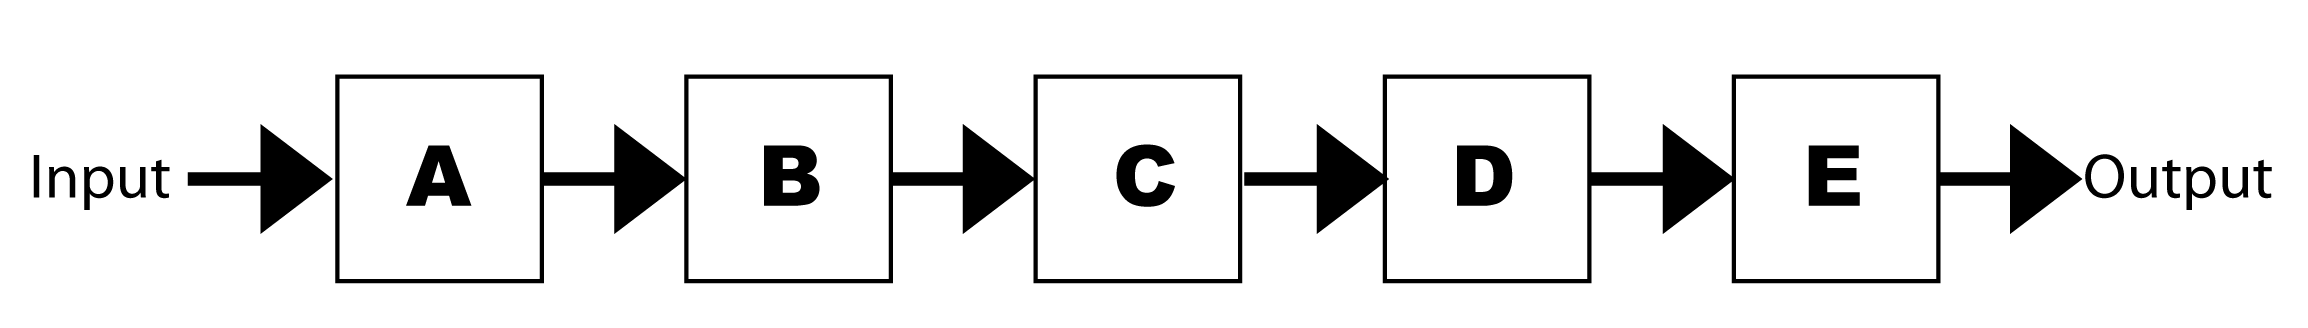
\includegraphics[scale=0.75]{ProjectAssignment1-1a.png}
					\end{center}
					\begin{enumerate}[A)]
						\item Initialize ACIDS
						\item Position METAL-V in search space
						\item Search for IEDs
						\item Determine if time is up
						\item Return ACIDS to ready state
					\end{enumerate}
				\item In order to achieve a system reliability of 0.90, the reliability allocation for RF3 is approximately 0.940.
					\begin{align*}
						x &= \frac{0.90}{0.988\times 0.974\times 0.999\times 0.995} \\
						&= \frac{0.90}{0.9574} \\
						&= 0.940
					\end{align*}
				\item The associated MTBF is $16.\overline{66}$ hours.
					\begin{align*}
						\lambda &= 1 - 0.940 \\
						\&= 0.060 \\
						\mbox{MTBF} &= \frac{1}{0.060} \\
						&= 16.\overline{66}
					\end{align*}
			\end{enumerate}
		\item % Question 2
			\begin{enumerate}
				\item It is given in the problem description that only the Vehicle Operator and the MVS are required to perform \emph{Function 3}.  These subsystems are not mutually redundant.  Consequently, the reliability network of the ACIDS subsystems \emph{required} for \emph{Function 3} is
					\begin{center}
						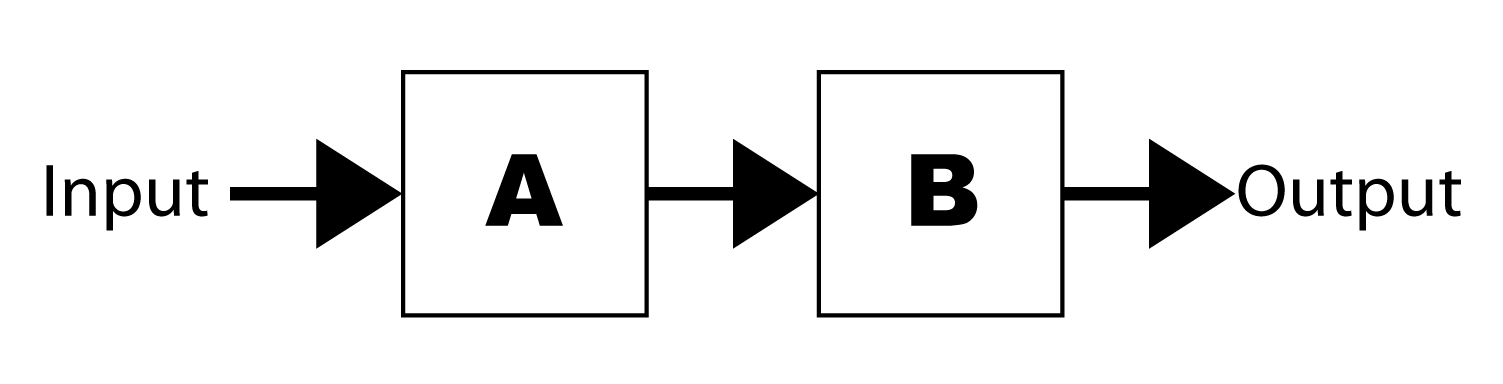
\includegraphics[scale=0.75]{ProjectAssignment1-2b.png}
					\end{center}
					\begin{enumerate}[A)]
						\item Vehicle Operator
						\item MVS
					\end{enumerate}
				\item Using the value calculated in 1b (above), the required reliability of the METAL-V subsystem would have to be 0.9592.
					\begin{align*}
						0.940 &= 0.980 \times x \\
						x &= \frac{0.940}{0.980} \\
						&= 0.9592
					\end{align*}
				\item The associated MTBF is 24.51 hours.
					\begin{align*}
						\lambda &= 1 - 0.9592 \\
						\&= 0.0408 \\
						\mbox{MTBF} &= \frac{1}{0.0408} \\
						&= 24.5098
					\end{align*}
			\end{enumerate}
		\item % Questiion 3
			\begin{enumerate}
				\item We should disregard the MVS Storage Container in relation to \emph{Function 3} since it is not utilized as part of that function.\footnote{Slide \#19.}
				\item Shown in the diagram below is the reliability network for the MVS components required for \emph{Function 3} where \emph{Function 3} is broken down as given in the project documentation.\footnote{Ibid.}
					\begin{center}
						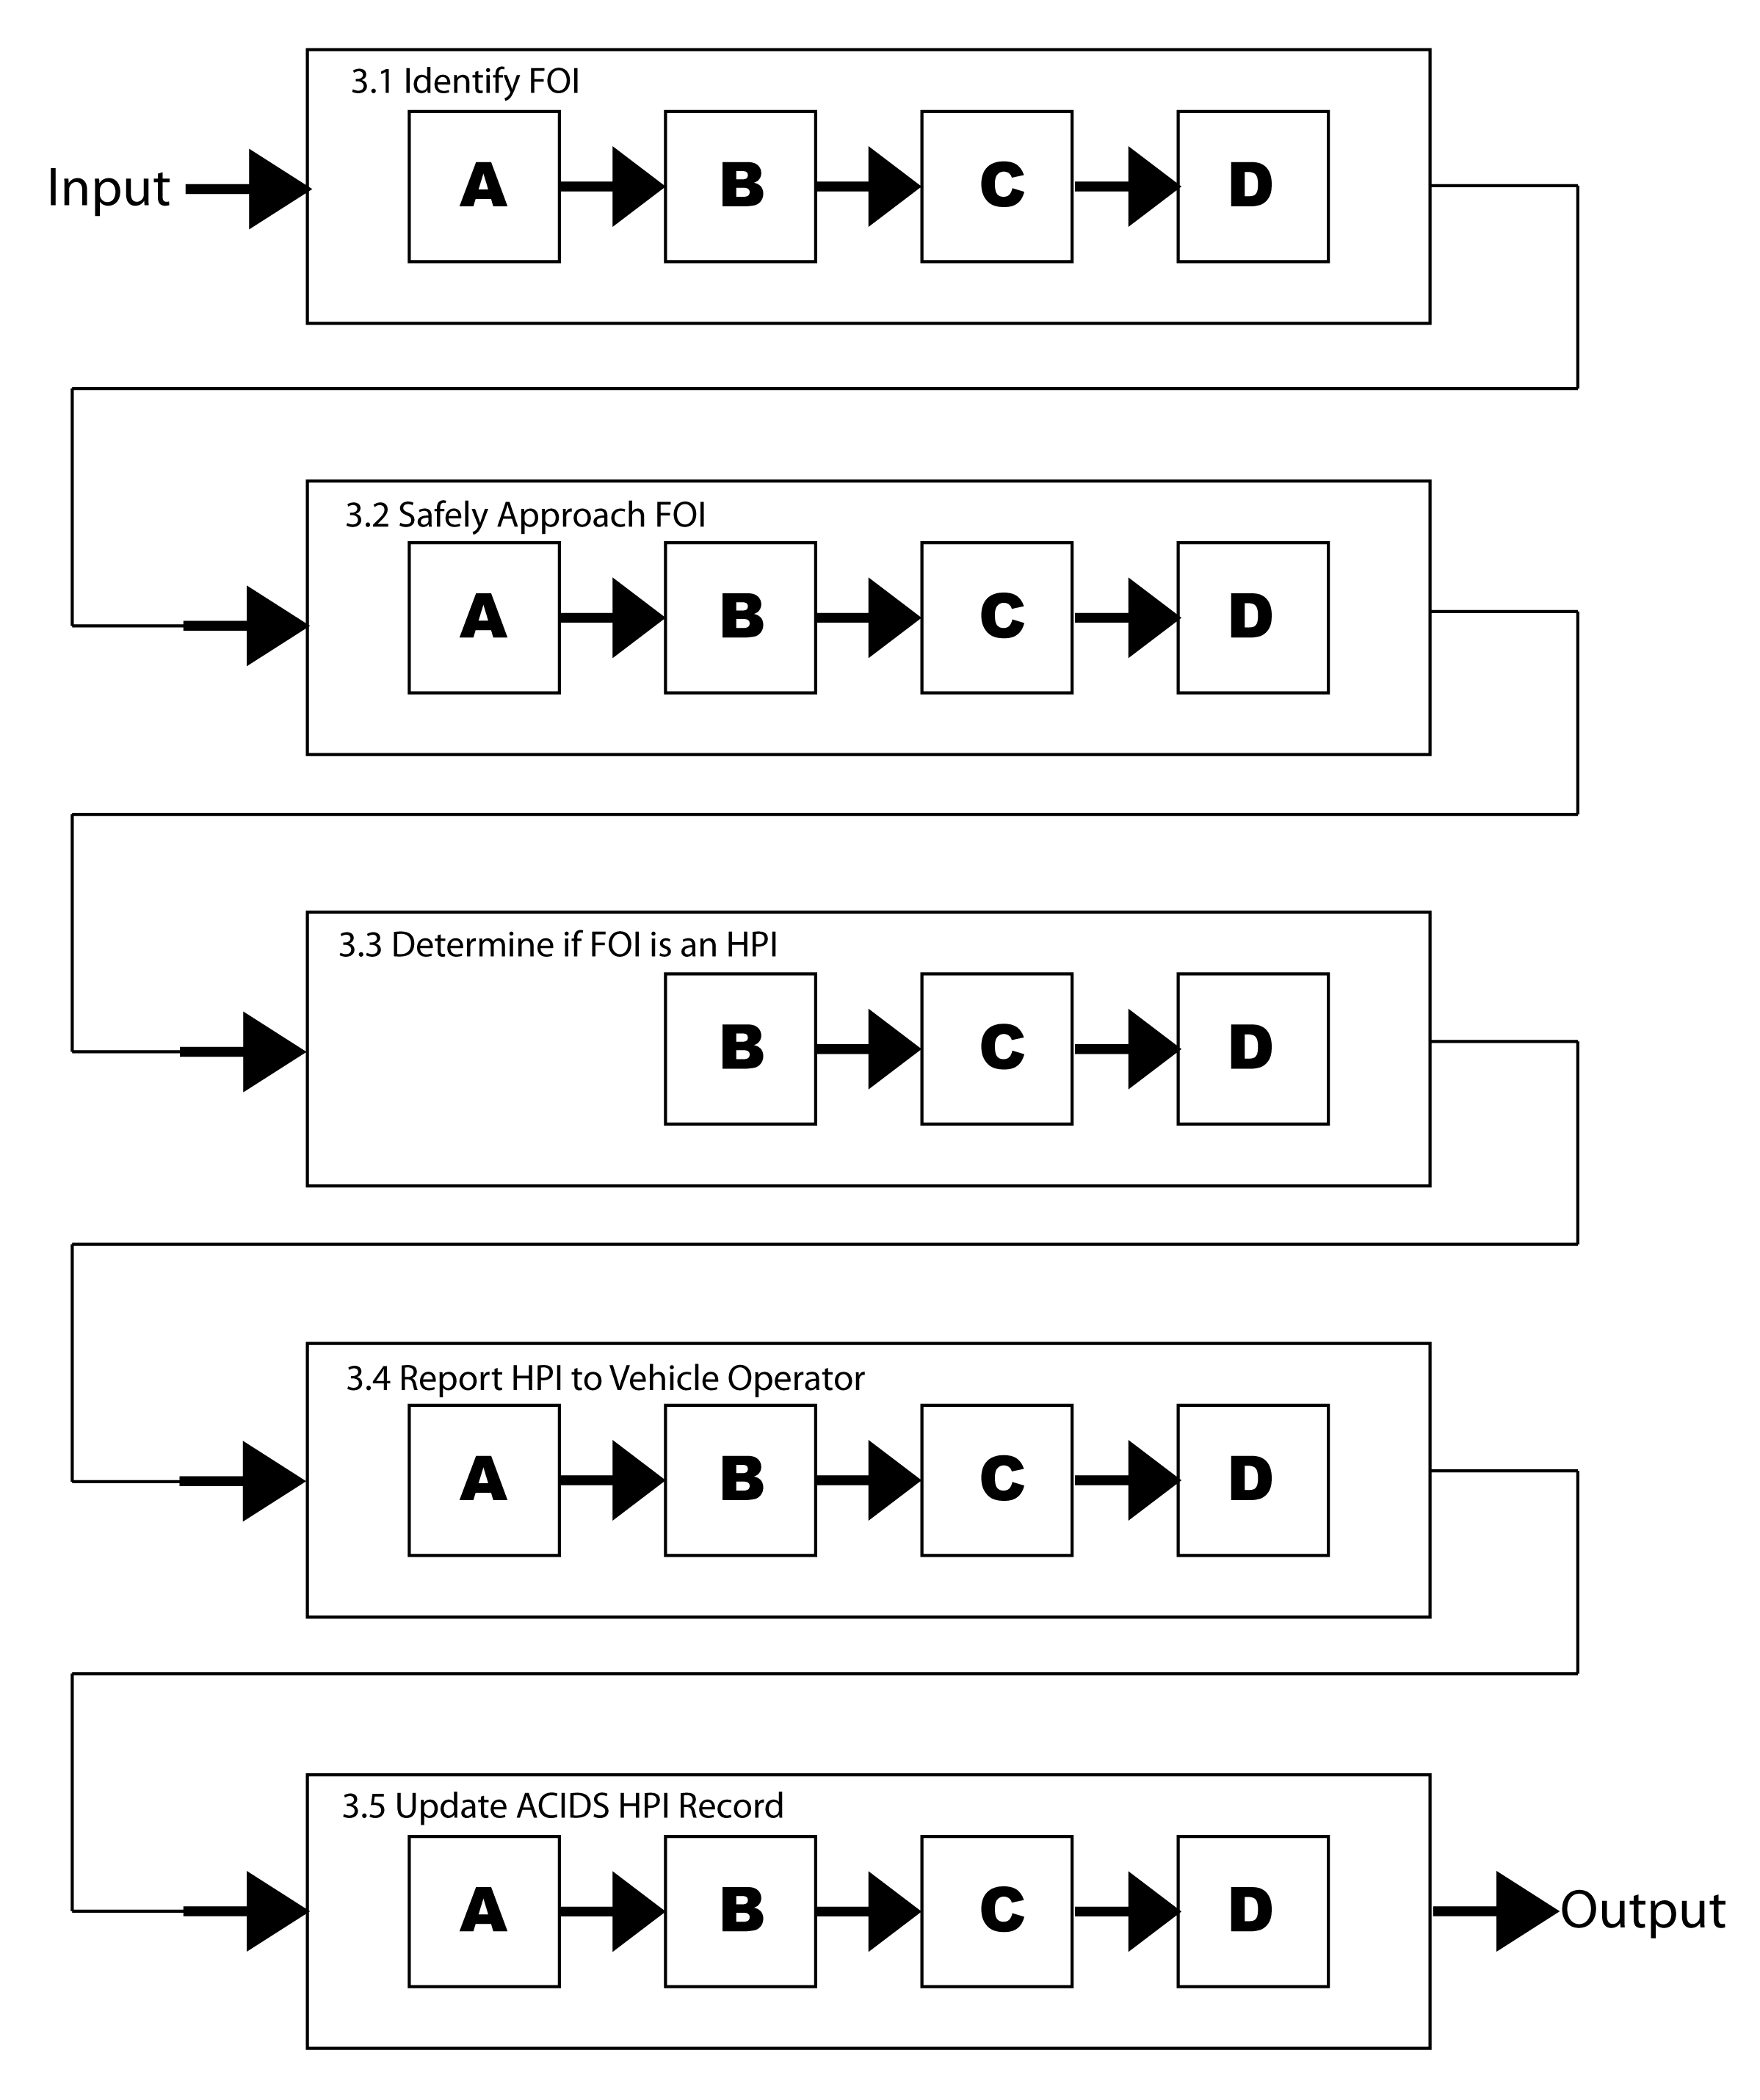
\includegraphics[scale=0.75]{ProjectAssignment1-3b.png}
					\end{center}
					\begin{enumerate}[A)]
						\item MVS Remote Controller
						\item METAL-V
						\item MVS Operational Software
						\item MVS Firmware
					\end{enumerate}
				\item Since the MVS Storage Container is not used in \emph{Function 3}, the derived reliability requirement for METAL-V is 0.9708.
					\begin{align*}
						0.9592 &= x\times 0.990\times 0.999\times 0.999 \\
						&= 0.9880x \\
						x &= \frac{0.9592}{0.9880} \\
						&= 0.9708
					\end{align*}
				\item The associated MTBF is 34.25 hours.
					\begin{align*}
						\lambda &= 1 - 0.9708 \\
						\&= 0.0292 \\
						\mbox{MTBF} &= \frac{1}{0.0292} \\
						&= 34.2466
					\end{align*}
			\end{enumerate}
		\item % Question 4
			\begin{enumerate}
				\item The diagram below depicts the reliability network for the METAL-V(1) for \emph{Function 3}.
					\begin{center}
						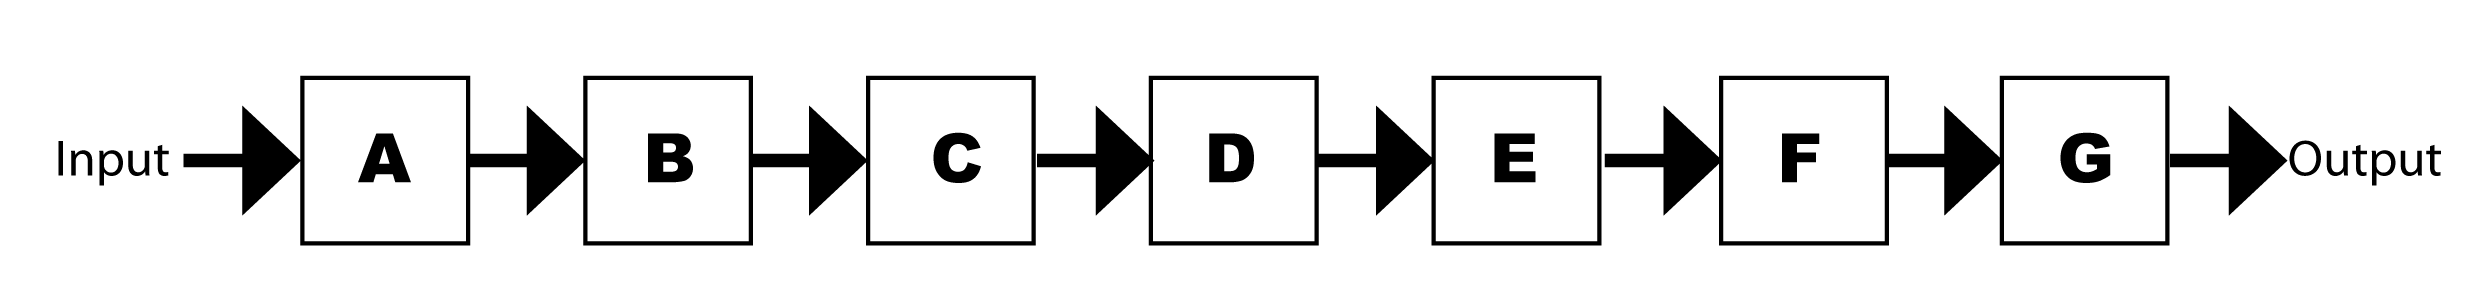
\includegraphics[scale=0.75]{ProjectAssignment1-4a.png}
					\end{center}
					\begin{enumerate}[A)]
						\item Drive Train
						\item Motor Set
						\item Chassis
						\item Computer Controller
						\item Communications Set
						\item Power Supply
						\item IED Sensor
					\end{enumerate}
				\item The reliability required for non-IED-sensor components as a block is 0.9776.
					\begin{align*}
						0.993x &= 0.9708 \\
						x &= 0.9776
					\end{align*}
					We could assign an identical reliability of 0.9962 to each of the 6 non-IED-sensing components.
					\begin{align*}
						x^{6} &= 0.9776 \\
						x &= \sqrt{0.9776} \\
						&= 0.9962
					\end{align*}
					This would result in a MTBF of 263.16 hours for each of the non-IED-sensor components.
					\begin{align*}
						\lambda &= 1 - 0.9962 \\
						&= 0.0038 \\
						\mbox{MTBF} &= \frac{1}{0.0038} \\
						&= 263.1579
					\end{align*}
				\item The diagram below depicts the reliability network for the METAL-V(2) for \emph{Function 3}.
					\begin{center}
					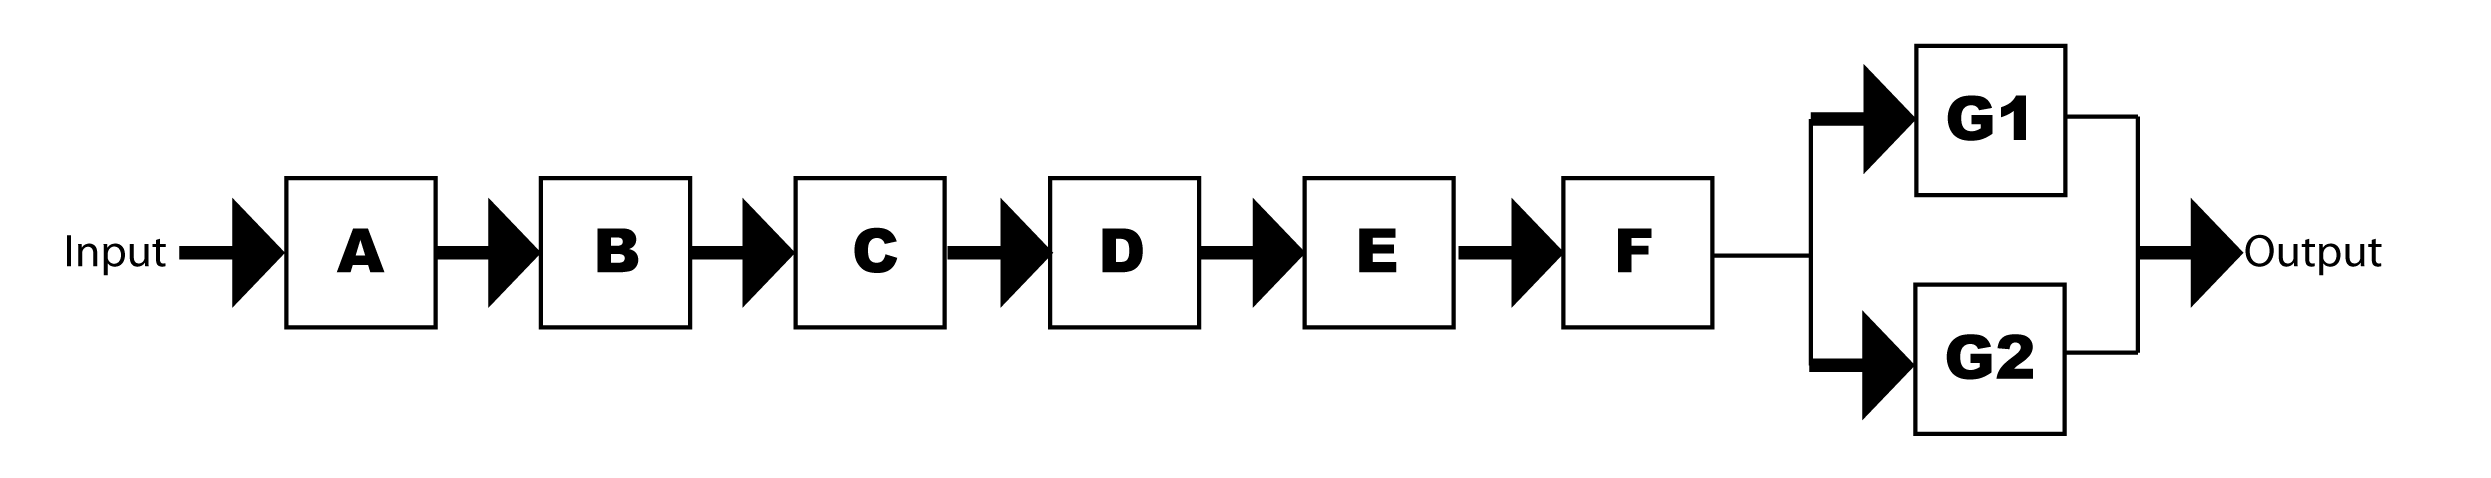
\includegraphics[scale=0.75]{ProjectAssignment1-4c.png}
						\end{center}
					\begin{enumerate}[A)]
						\item Drive Train
						\item Motor Set
						\item Chassis
						\item Computer Controller
						\item Communications Set
						\item Power Supply
						\item IED Sensors
					\end{enumerate}
				\item The reliability required for non-IED-sensor components as a block is 0.9708.  The reliability of the redundant sensor block is calculated as
					\begin{align*}
						\mbox{RSEN2} &= 1 - ((1 - 0.993)(1 - 0.993)) \\
						&= 1 - (0.007)^{2} \\
						&= 1 - 0.000049 \\
						&= 0.999951
					\end{align*}
					And we calculate the reliability required for the non-IED-sensor components as
					\begin{align*}
						0.999951x &= 0.9708 \\
						x &\approx 0.970847572 
					\end{align*}
					We could assign an identical reliability of 0.9951 to each of the 6 non-IED-sensing components.
					\begin{align*}
						x^{6} &= 0.9708 \\
						x &= \sqrt{0.9708} \\
						&= 0.9951
					\end{align*}
					This would result in a MTBF of 202.97 hours for each of the non-IED-sensor components.
					\begin{align*}
						\lambda &= 1 - 0.9951 \\
						&= 0.0049 \\
						\mbox{MTBF} &= \frac{1}{0.0049} \\
						&= 202.9650
					\end{align*}
			\end{enumerate}
		\item Given a sufficient understanding of the engineering problem and accurate data from which to start, reliability analysis, design, and engineering can be built up beginning with a case which is much easier to understand.  Then, gradually adding complexity, the problem can be better understood, predicted, and trade-offs can be made with regard to cost, time, and reliability.
		\item 
			% Describe the problem
			There are two aspects to clearing imrovised explosive devices (IEDs) in theater.  The first, and more thoroughly addressed, is to clear routes and the second is to clear areas.  Leveraging the prototype system, Micro Expeditionary Transforming Air Land-Vehicle (METAL-V), we will formulate a better understanding of the engineering problem space associated with fielding a similar vehicle.  We will restrict the scope of this project to ground vehicle solutions and defer flight aspects.  The METAL-V is the centerpiece of the Advanced Counter IED Detection System (ACIDS).  The entire ACIDS system consists of a vehicle operator, the METAL-V subsystem, a programming unit, a programming unit operator, and an ACIDS diagnostic subsystem.
			\par Area clearing of IEDs means simply that a well-bounded area is searched, IEDs are located, marked, and removed, and the search vehicle is returned to a known good state.  This activity shall result in the identificaiton and removal of all IEDs in the given area and shall be comleted within two (2) hours.
			% Describe the system
			\par We will be using a derivative of the prototype METAL-V system in simulation, called \emph{Simulated} METAL-V (SMETAL-V).  It shall consist of a remote controller, a storage container, the METAL-V hardware, firmware, and operational software.  The METAL-V, itself, is comprised of a drive train, motor set, chassis, computer controller, communications set, power supply, and one or more IED sensors.
			% Outline the method to solve the problem
			\par Locating and clearing IEDs shall work as follows.  First, the programming unit operator will initialize ACIDS then the vehicle operator will position the METAL-V subsystem within the designated search area.  The METAL-V will search for IEDs within the bounded area until all IEDs are located or until the mission time has expired.  Lastly, ACIDS is returned to the ready state.  When a potential IED is located it is first safely approached and further inspected to determine if it is likely to actually be an IED.  If it is determined to be, then it is reported to the ACIDS operator and the ACIDS records are updated accordingly.  The IED is then cleared and the search continues.
			% Discuss design trade-offs
			\par During our design analysis for reliability we determined that we could benefit from redundant IED sensors.  This increases the reliability of the sensors from 0.993 for one to 0.999951 which eases the requirement somewhat for non-IED-sensor components of METAL-V.  Specifically it allows us to reduce the mean time between failure for non-IED-sensor components from 263 hours to approximately 203 hours while still maintaining the same overall reliability of 0.9708 for the METAL-V sybsystem.
			% Summarize and draw a conclusion about the solution
	\end {enumerate}
\end{document}